\documentclass[14pt]{article}

\title{\textbf{Interactive graphics: a simple Babylon.js game}}
\author{Andrea Del Vecchio 1749574\\
		delvecchio.1749574@studenti.uniroma.it}

\usepackage[utf8]{inputenc}
\usepackage{float,graphicx,amsmath,wrapfig}
\usepackage{hyperref}

%For indentation
\newlength\tindent
\setlength{\tindent}{\parindent}
\setlength{\parindent}{0pt}
\renewcommand{\indent}{\hspace*{\tindent}}


\date{}

\begin{document}
\maketitle
\section{Introduction}
The aim of this project is to implement a very simple game using Babylon.js. The game uses mainly Babylon js and the Babylon js 3D GUI. A number of interactions are available (enabling/disabling the sound, changing difficulty, opening the main menu) to make the game \textit{interactive}. The project has been tested on mozilla firefox and microsoft edge. In order to properly run it, be sure to have a web browser that supports WebGL 2.0 and an up to date javascript interpreter since classes are widely used. To directly jump to the game description go to the section \ref{sec:theGame} The Game. To know a little more about the technical solutions implemented read \ref{sec:technicalManual} The framework.
\section{The framework}\label{sec:technicalManual}
Babylon is a very powerful framework which offers an high level API to create 3D graphic programs that run on web browsers. It is very easy and guarantees GPU hardware acceleration freeing the user from the burden of directly programming the shaders. Babylon js uses a powerful rendering system which automatically computes the world and model view matrices considering the cameras and the object present in the scene. It also offers a set of API that serves the purpose of defining light sources which can be point lights, directional lights, spotlights or hemispherical lights for example. Objects in the scene can be equipped with materials which will react differently to the different components of the light sources. \\
Babylon.js offers also a powerful system that can be used to synchronize the loading process of each element in the scene through the \textit{assets manager}. The assets manager can be istantiated to import the sound and the desired meshes right before the actual scene is rendered so that the player never experience a \textbf{partial rendered scene}. With the asset manager, we can stack a set of tasks which will be executed one after the other. After executing a task in the stack, the asset manager will execute a callback function. We then associate to each loading process a separate task. To exploit this mechanism we can modify the asset manager to render the scene only when executing the last stack element callback.\\
The core of a Babylon js system is undoubtedly the \textbf{engine}. An engine is responsible of loading the scene and handles the render loop, in which it renders the scene vertices and execute functions. The scene, on the other hand, wraps all the objects that are used to effectively create the level, all of which are rendered in each iteration of the render loop \footnote{\url{https://doc.babylonjs.com/api/classes/babylon.scene}.}.\\
To handle scene object interaction Babylon.js provides an handy interface called ActionManager. The action manager contains a set of triggers which can be set to execute actions when a certain event happens. For example, when two meshes instersect and the action manager is activated, a special kind of event is triggered and a callback fuction is executed. This system is exstensively used to create the shooting system in the game. The trigger should be considered as a simple test which returns a boolean value. The action will be performed if and only if the result of the test is true. There are many type of actions defined by the Babylon.js API: some might set certain values of an object property, some others may execute code that will alter the status of the scene.\\
Each scene is represented by a Babylon.Scene istance. To fully exploit Babylon modularity, we assign to each level a scene object.\\
To create animations, the programmer may use the babylon Animation object which, among other things, makes possible to define key frame animations, a powerful yet easy to use paradigm to define animations \footnote{\url{https://doc.babylonjs.com/babylon101/animations}.}. \\
Babylon.js allows also the user to include a special object in their project, called \textit{particle system}. A particle system can be used in different scenarios to simulate water flows or blood coming out from wounds. In this case the particle system has been used to simulate fire. It is quite simple to use. You mainly need to specify the mesh source, an emission rate, the emission direction and the eventual texture or colour applied to the particles.\\
A particle is indeed a very small cube. So it is possible to set a colour and a texture to it. The \textit{emit rate}, on the other hand, specifies how many particles are generated per second from a given source. The user may also specify a minimum and a maximum lifetime for the particles 
\footnote{\url{https://doc.babylonjs.com/babylon101/particles}.}.\\

To render the main menu and the player status information, we use the Babylon.js 3D GUI. Each element in a Babylon GUI is associated to special kind of texture which is called \textbf{ texture}. An advanced texture could be concieved as a container which can store other GUI elements like buttons, checkboxes or textblocks or GUI panels. The panels are lower level containers which can contain other elements in a hierarchical way. Defining a GUI with Babylon.js is relatively straightforward and most importantly, the advanced texture is just an element of the scene, so it does not cause any conflicts with other scene objects.\\

\section{The environment}
\subsection{Description}
The scene level is very simple. It is a flat 2000x2000 map placed somewhere in the space that represents an arena. In this scenario two team of tanks fight to the death: the \textbf{red} and the \textbf{blue} team tanks. \\
\begin{figure}[H]
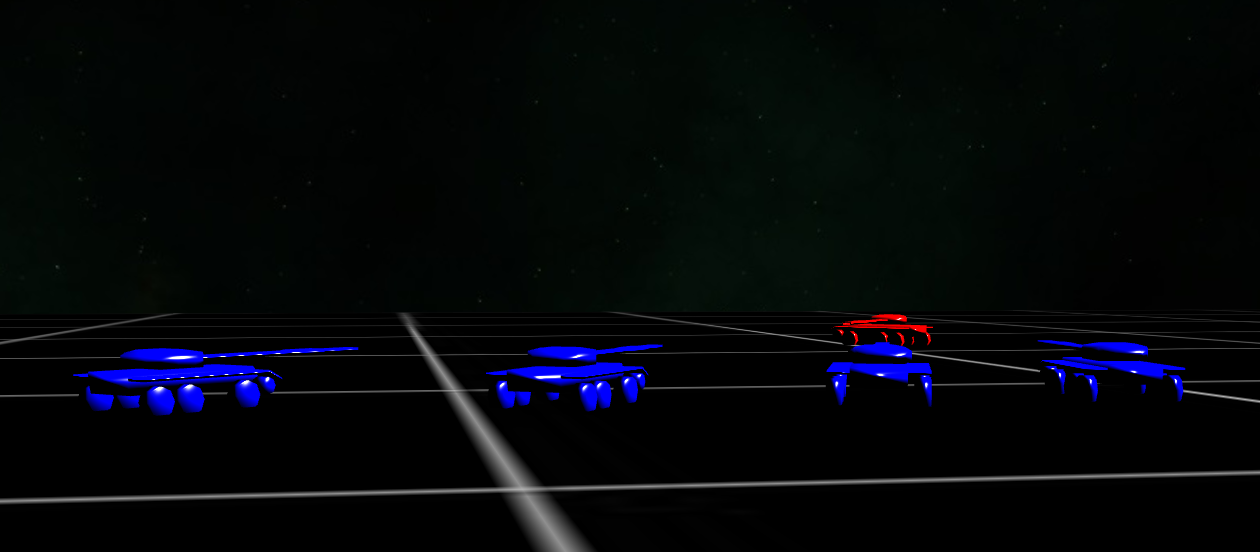
\includegraphics[width = 12cm]{images/scenario3.png}
\caption{Overview of the fighting arena. The red tank and the blue tanks fight to the death.}
\label{img:scenario}
\end{figure}



The player plays as a red team tank and he is the only member of its team. He is able to move in the map with its tank collecting bonuses from the loot boxes and shooting towards the opponent tanks. The scenario is brightened by a white directional light  simulating a nearby star or a big reflector. The map is completely flat, so the player tank do not need to worry about the uneven ground.\\

\begin{figure}[H]
\begin{minipage}[t]{0.45\textwidth}
\center
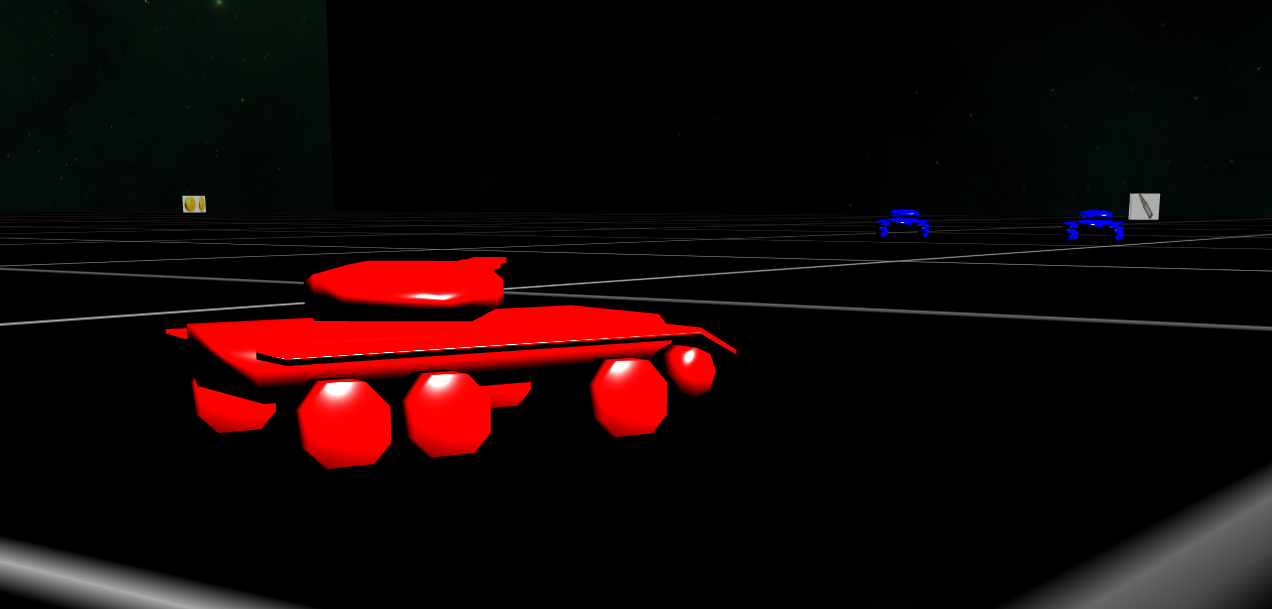
\includegraphics[width=\textwidth]{images/scenario.png}
\end{minipage}
\hfill
\begin{minipage}[t]{0.45\textwidth}
\center
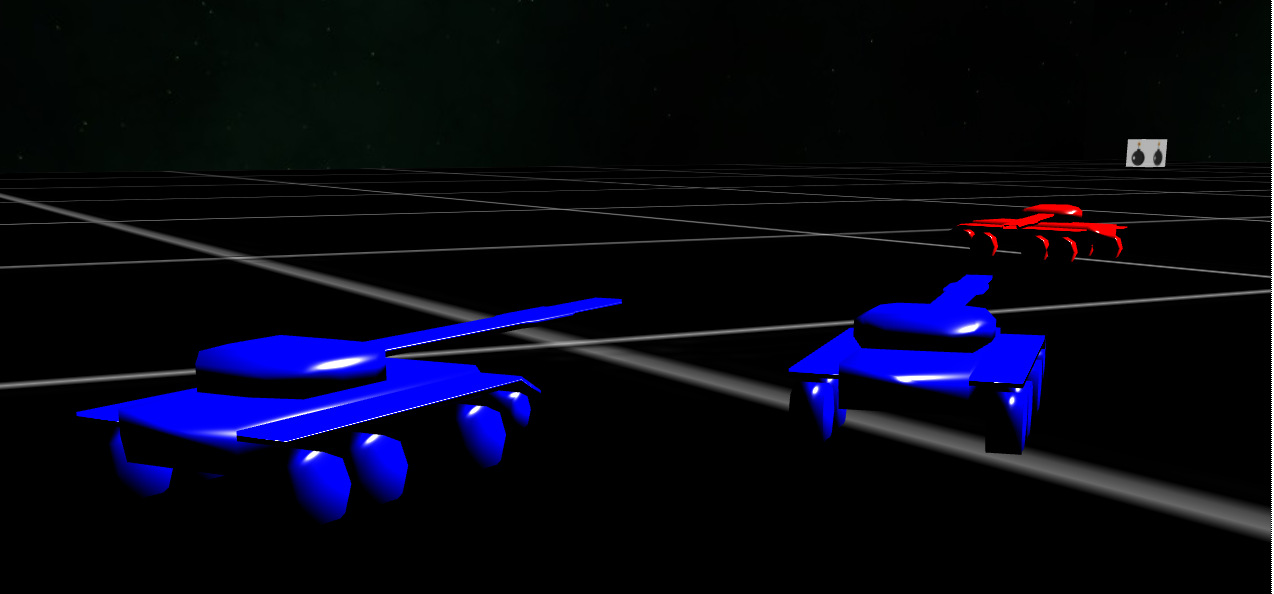
\includegraphics[width=\textwidth]{images/scenario2.png}
\end{minipage}
\label{img:scenario2}
\end{figure}
The ground is equipped with a very simple physic mechanism that allows the physical objects to dinamically interact with it. It has no borders so the player needs to be careful not to move outside the map otherwise he will be teleported to its spawn position.
\subsection{Implementation details}
To completely render the scene, Babylon js forces the program to create a camera. So at least a camera must be specified. Since we need an external third person shooter camera or a \textit{external} vehicle camera, we created a \textbf{follow camera} object.
\begin{figure}[H]
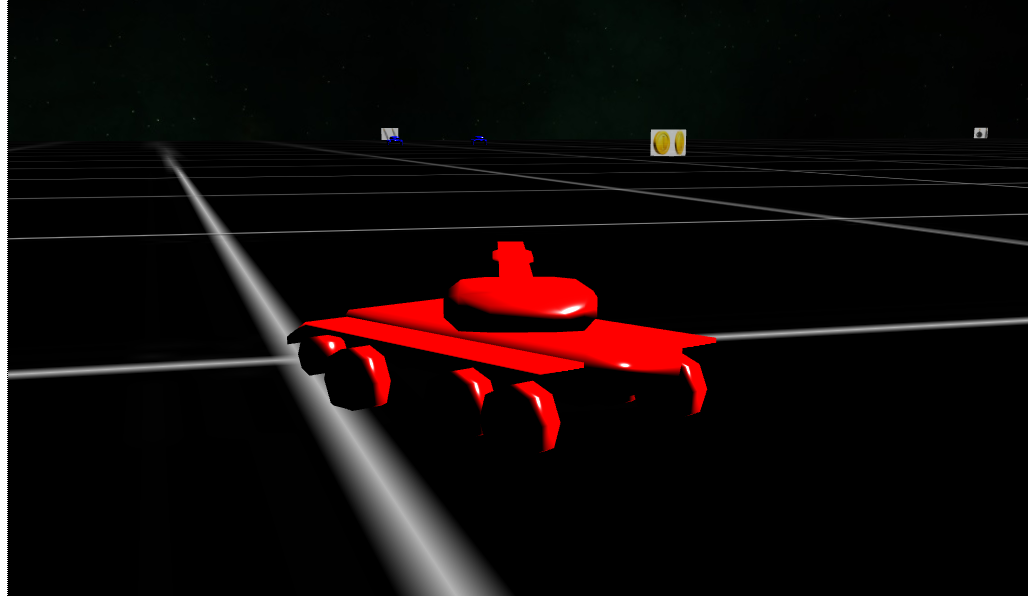
\includegraphics[width = 12cm]{images/thirdPerson.png}
\caption{Overview of the third person shooter camera.}
\label{img:thirdPerson}
\end{figure}
The follow camera is a powerful tool available in Babylon js framework. The camera needs a target mesh to follow and can be tuned with a variety of parameters. In order to make the player able to drive the red tank, we set the tank as the target of the follow camera \footnote{Since the tank is a hierarchical model imported from the web, the camera is attached to the \textbf{root} of the tank.}. The API also make possible to attach the camera to the HTML canvas so that the user can directly control with the mouse and the keyboard arrow buttons, so we attached the follow camera to the canvas. \\
Moreover HTML 5 provide a useful feature when it comes to program an interactive game: the \textbf{pointer lock}. With this feature, the canvas are able to \textit{capture} the mouse pointer so that the user cannot click outside it causing undesired effects (for example closing the browser window by mistake terminating the game).

\begin{figure}[H]
\center
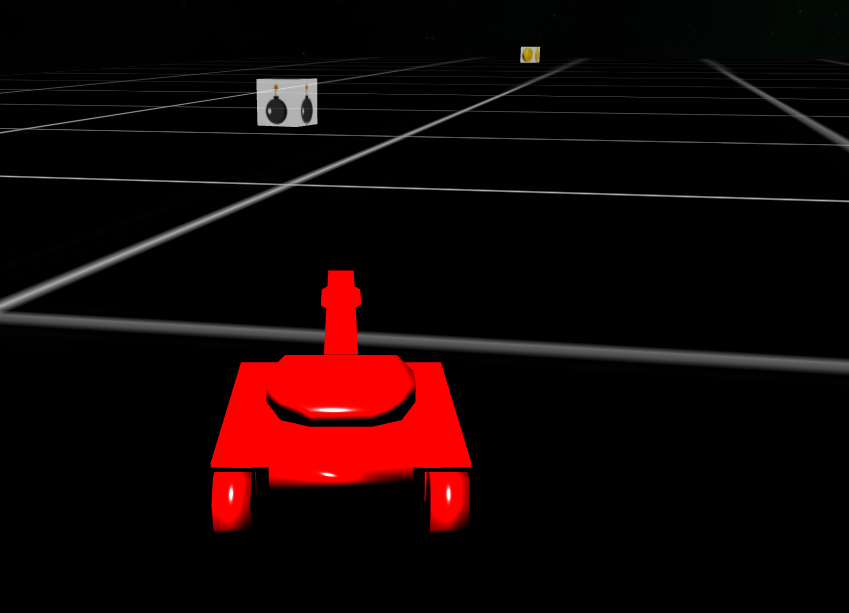
\includegraphics[width = 12cm]{images/lootBoxes.png}
\caption{The scene in easy mode with two of the nine loot boxes. Near the tank, a cannon ball loot box and in the background a point loot box.}
\label{img:lootBoxes}
\end{figure}

The user then, can get full control of the mouse by simply clicking the \textit{Esc} keyboard button.\\
Depending on the chosen difficulty, which can be either \textbf{easy} or \textbf{hard}, the engine will render 9 or 6 loot boxes [figure \ref{img:lootBoxes}]. The boxes are texturized using the advanced \textit{cube texturing} mechanism provided by Babylon.js which is also used to create skyboxes. To attach a cube texture to an object six images which corresponds to the six faces of the cube are needed. The images must be placed in the same directory and needs to have a \textit{common name} which is equal to each of the six images followed by \textit{position tag} which must be one of (px,py,pz,nx,ny,nz) \footnote{See \url{https://doc.babylonjs.com/resources/playground_textures\# cubetextures}}. \\
px, py, pz stands for \textit{positive} x,y,z. nx,ny,nz stands for \textit{negative}x,y,z. Each of the preeciding tags corresponds to a face of the box to be texturized. The position of each face follows the Babylon.js cube textures convention that is specified in the official documentation.\\
Each box is animated thanks to a \textbf{key frame animation}.
To create a key frame animation, you have to provide a list of javascript objects in the form 

\[\text{\{frame: value\}}\]

where the \textbf{frame} is a frame number and the \textit{value} field represents a possible value for the given property of the object at that frame. In this case the boxes are equipped with two key frame animations: the first one for its height and the second one for the rotation along the \textit{y} axis. The animation is is composed by 100 frames and runs at 10 frames per second so that the player has an impression that the boxes \textbf{floats} above the ground. This type of animation is inspired by the \textbf{Mario Kart}\textsuperscript{TM} floating boxes that contain the various bonuses for the players in the race.\\

\begin{figure}[H]
\begin{minipage}[t]{0.45\textwidth}
\center
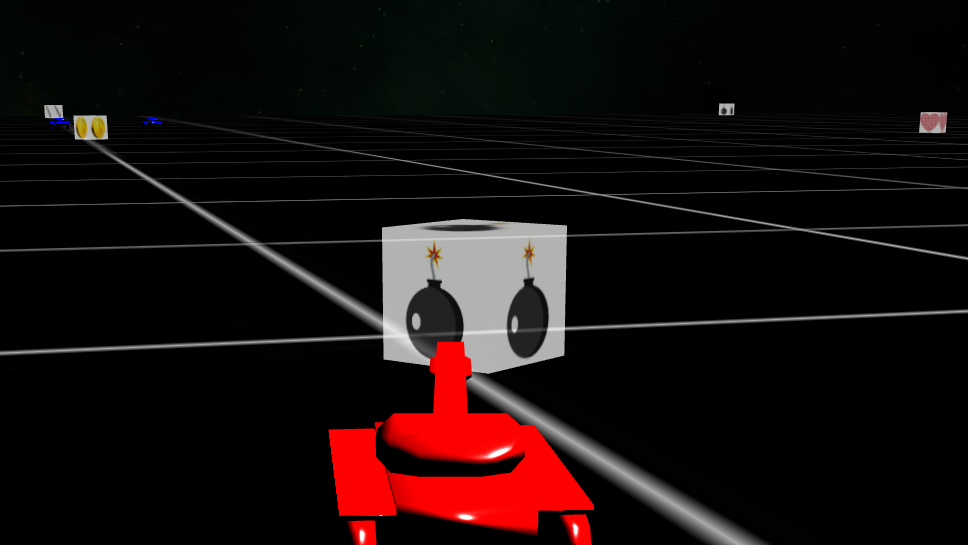
\includegraphics[width=\textwidth]{images/beforeLoot.png}
\end{minipage}
\hfill
\begin{minipage}[t]{0.45\textwidth}
\center
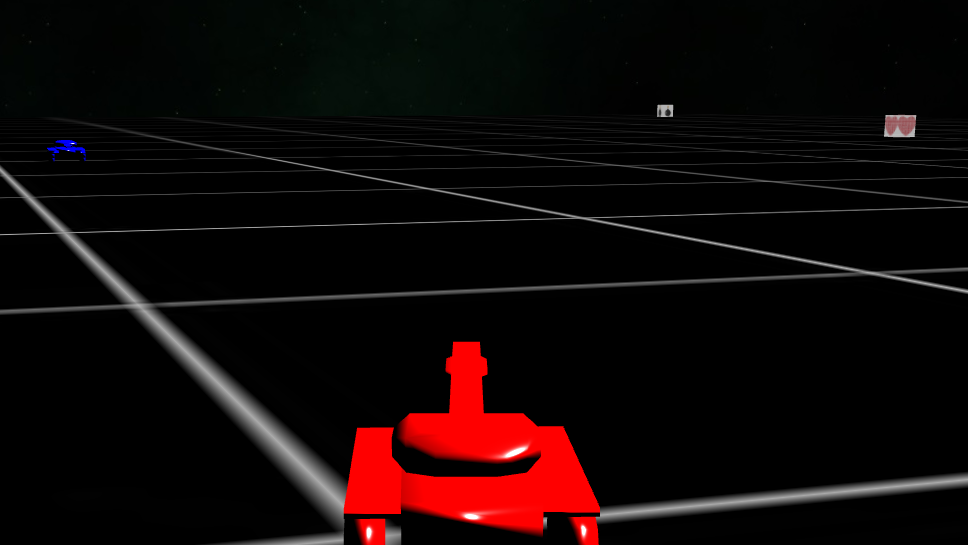
\includegraphics[width=\textwidth]{images/afterLoot.png}
\end{minipage}
\caption{The player tank before and after collecting the cannon ball loot boxes.}
\label{img:beforeAfterLooting}
\end{figure}


The boxes are associated to a Babylon.js trigger [figure \ref{img:beforeAfterLooting}]]. When the red tank, which from now on we call the \textbf{hero tank}, intersects one of the boxes, the box will disappear and the associated bonus is collected by the player. The loot box mesh is then destroyed to free some memory. Since the red and the blue tanks are composed by a considerable amount of vertices, we paid particular attention to free memory whenever it is possible to optimize the scene. Both the red and the blue tanks are composed by a considerable amount of vertices, so keeping in memory the position of unused objects which must not be rendered by the scene engine is a huge waste of computation resources. After a period of time of 5 seconds the boxes will respawn to their original positions and are ready to be collected again by the player and the corresponding vertices are recreated and passed to the GPU for rendering. \\
There are mainly four type of boxes:
\begin{itemize}


\item A \textbf{point box} represented by a big yellow coin. Collecting these boxes will make the player to earn a point. The amount of points a player has collected so far is shown in the top left corner of the screen. Since opponent tanks will keep spawning, collecting points is crucial to complete the game and obtain the \textbf{win condition}. 
\item A \textbf{machine gun box} represented by a big machine gun bullet. Collecting those boxes is not vital but it allows the player to obtain 10 additional machine gun bullets. The machine gun can be used to kill the opponent tanks.

\item A \textbf{cannon box} represented by a big cannon ball. Collecting those boxes is not mandatory to win the game but it is still useful as it allows the player to collect 2 additional cannon balls. Cannon balls can be used to kill opponent tanks and deals more damage than machine gun bullets.

\item A \textbf{health box} represented by a big hearth. Picking the health boxes could be a good strategy to play a safe game since the opponent tanks are very aggressive and constantly try to shoot towards the player tank to hunt it down. Collecting health boxes guarantees the player 3 additional life points until a certain maximum amount of life points is reached.

\end{itemize}

At any time during the game the player can go to the main menu by simply pressing the \textit{m} button. This will cause the current game to terminate and the corresponding scene to be disposed. From the main menu the player is able to change the difficulty of the game, to enable or disable the sound or to start a brand new game.\\
The environment has also a skybox. The texture of the skybox is taken from the official babylon js documentation and attached as a cube texture to a big box that surrounds the scene.

\section{The tank model}
\subsection{The hierarchical model}
The tank model is imported from a website which contains a series of free models that could be downloaded and used in Babylon.js projects \footnote{See also \url{https://clara.io/library?query=tank&gameCheck=true} for more information.}. 

\begin{figure}[H]
\center
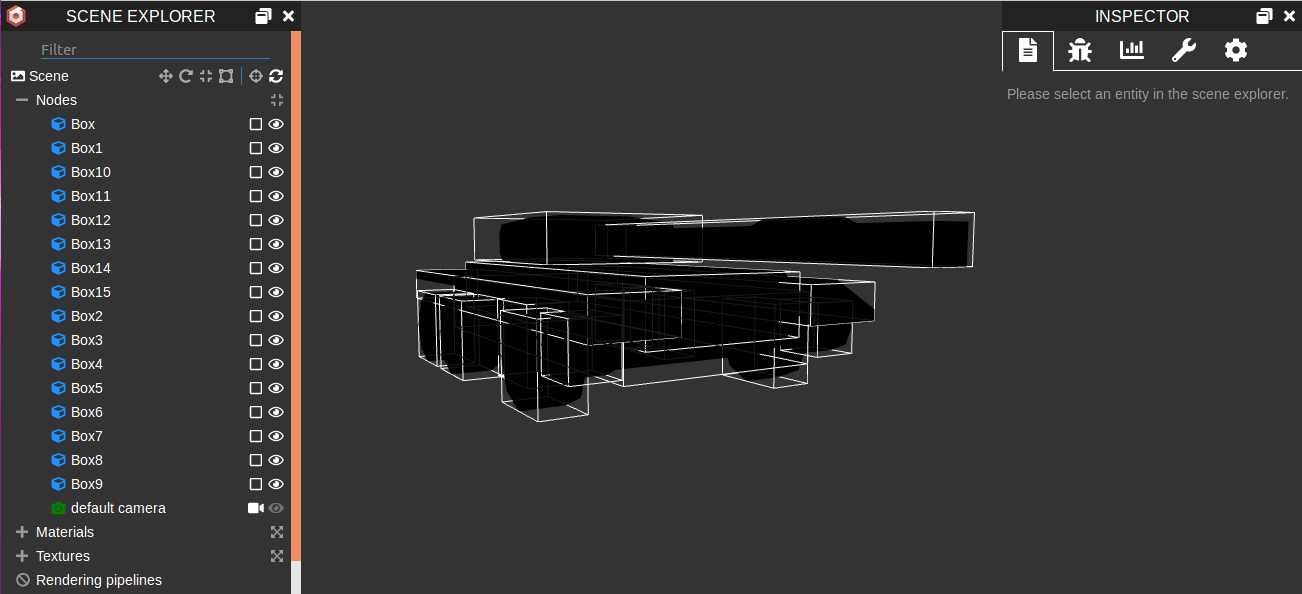
\includegraphics[width=12cm, height= 6.5cm]{images/model_sandbox.png}
\caption{The imported model viewed through the scene inspector of the Babylon.js sandbox. All the component meshes are highlilghted toghether with the corresponding names.}
\label{img:modelSandbox}
\end{figure}


The imported mesh is in a form of a set of unlinked boxes [figure \ref{img:modelSandbox} ]. It means that, at this stage, the tank is not a hierarchical model and managing it in the scene could be a challenging task.\\


\begin{figure}[H]
\center
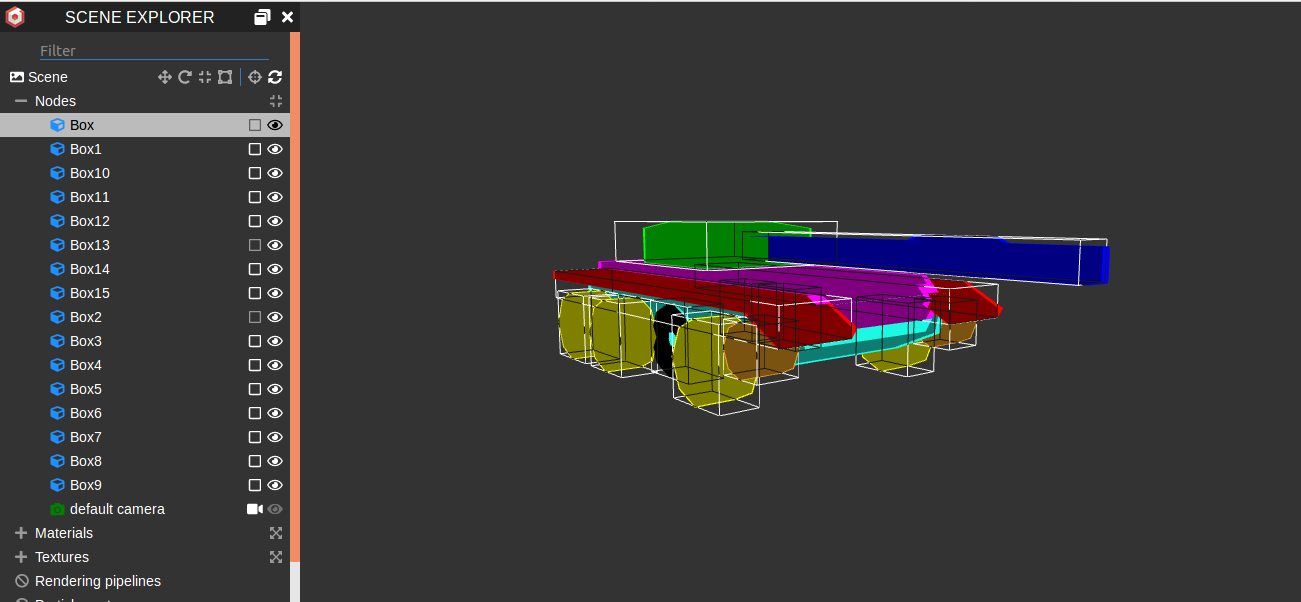
\includegraphics[width=12cm, height= 6.5cm]{images/evidencedModel.png}
\caption{The imported model viewed through the scene inspector of the Babylon.js sandbox with all the model components highlighted with different colours. We have then: the root in light blue, the body in purple, the turret in green, the cannon in blue, the wheels in yellow, the front wings in orange, the wings in red. The mesh in black has been discarded from the actual game for design purposes.}
\label{img:modelInspection}
\end{figure}



Fortunately Babylon.js implements a simple mechanism through the \textit{addParent, addChild, removeParent,removeChild} interface which is able to istantiate a hierarchical model on the fly [figure \ref{img:modelInspection} ]. The mechanism is built so that each transformation that is applied to the root of the model is also applied to the children. Then, whenever we have to move the tank, it is sufficient that we apply a translation to the root of the model instead of applying it to each component mesh which would be dramatically difficult in some scenarios.\\



\begin{figure}[H]
\begin{minipage}[t]{0.45\textwidth}
\center
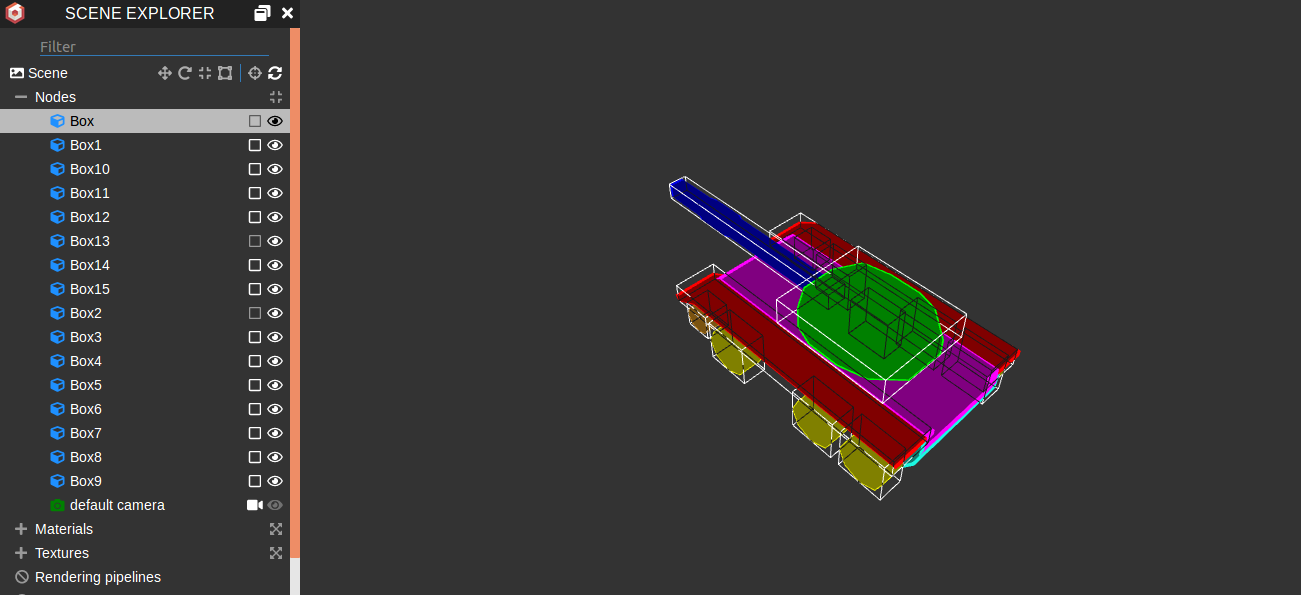
\includegraphics[width=\textwidth]{images/evidencedModel2.png}
\end{minipage}
\hfill
\begin{minipage}[t]{0.45\textwidth}
\center
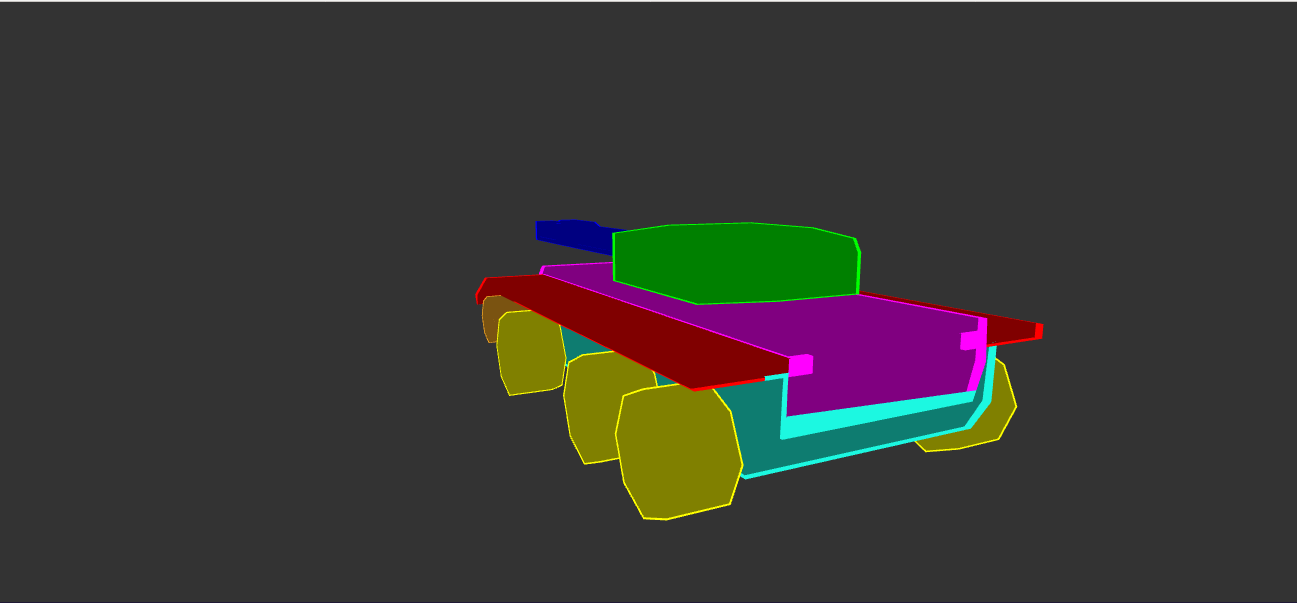
\includegraphics[width=\textwidth]{images/evidencedModel9.png}
\end{minipage}
\begin{minipage}[t]{0.45\textwidth}
\center
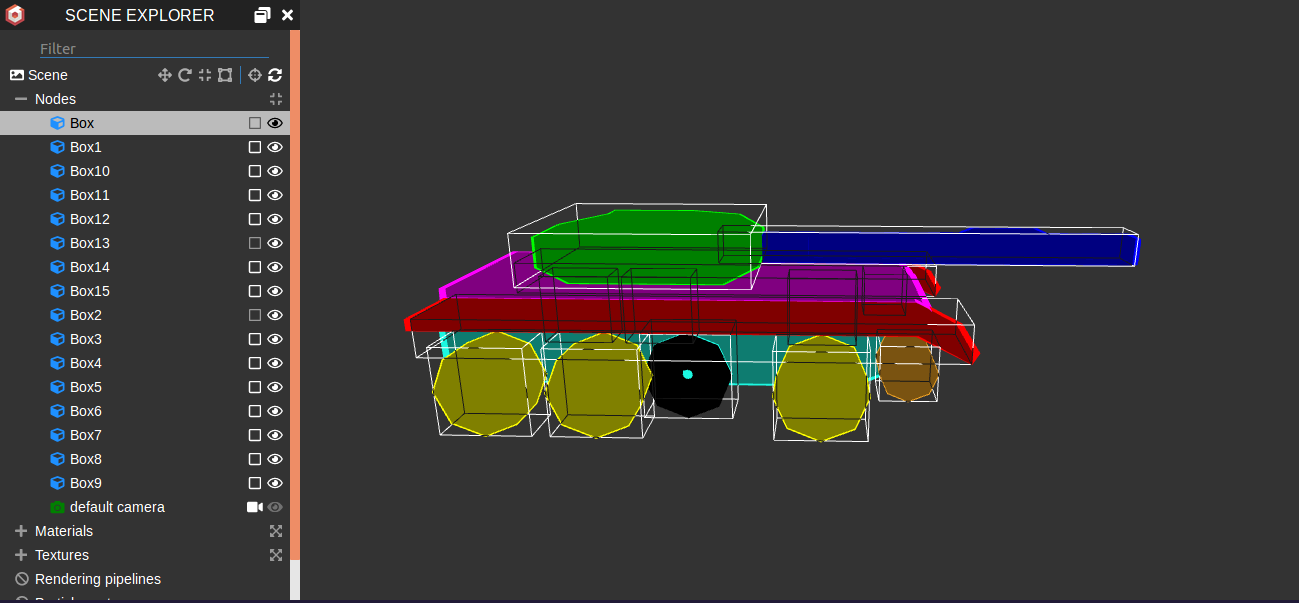
\includegraphics[width=\textwidth]{images/evidencedModel4.png}
\end{minipage}
\hfill
\begin{minipage}[t]{0.45\textwidth}
\center
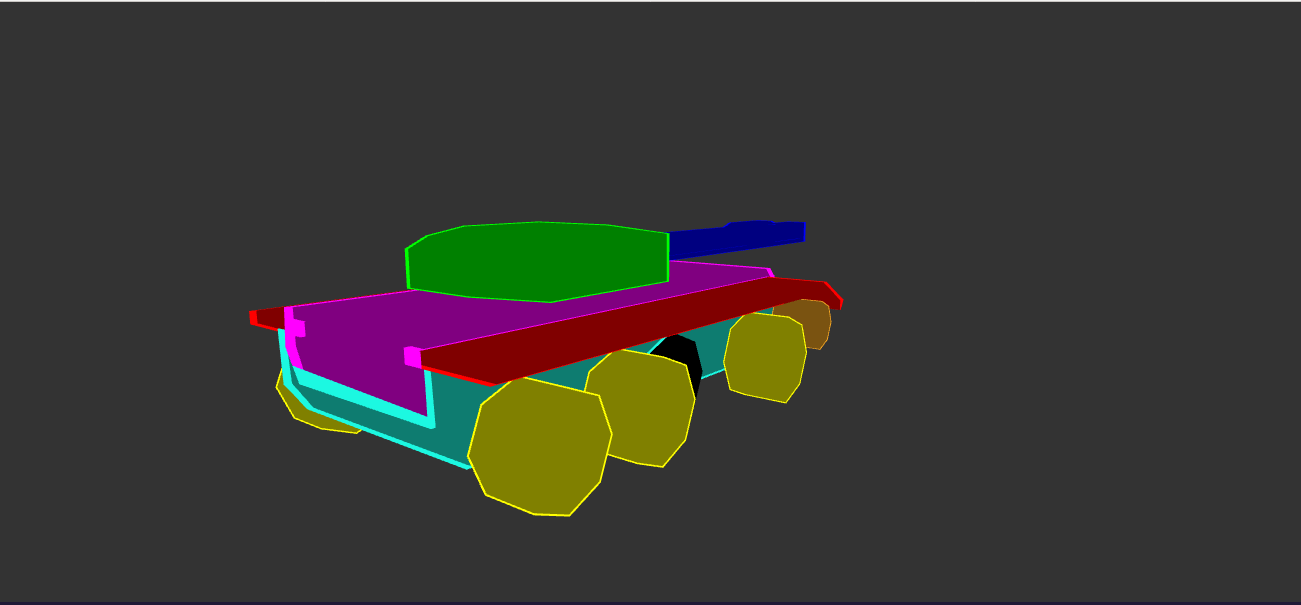
\includegraphics[width=\textwidth]{images/evidencedModel11.png}
\end{minipage}
\caption{Two views of the different components of the tank model.}
\label{img:modelInspection2}
\end{figure}


For simplicity, I decided to set the mesh named \textbf{"Box"}(the mesh in light blue) as the root of the model. All the pieces, apart from the cannon, are set as its \textit{children} whereas the cannon is set as a child of the turret (the green mesh)[figure \ref{img:modelInspection2} ].
\subsection{Animating the turret}

\begin{figure}[H]
\begin{minipage}[t]{0.45\textwidth}
\center
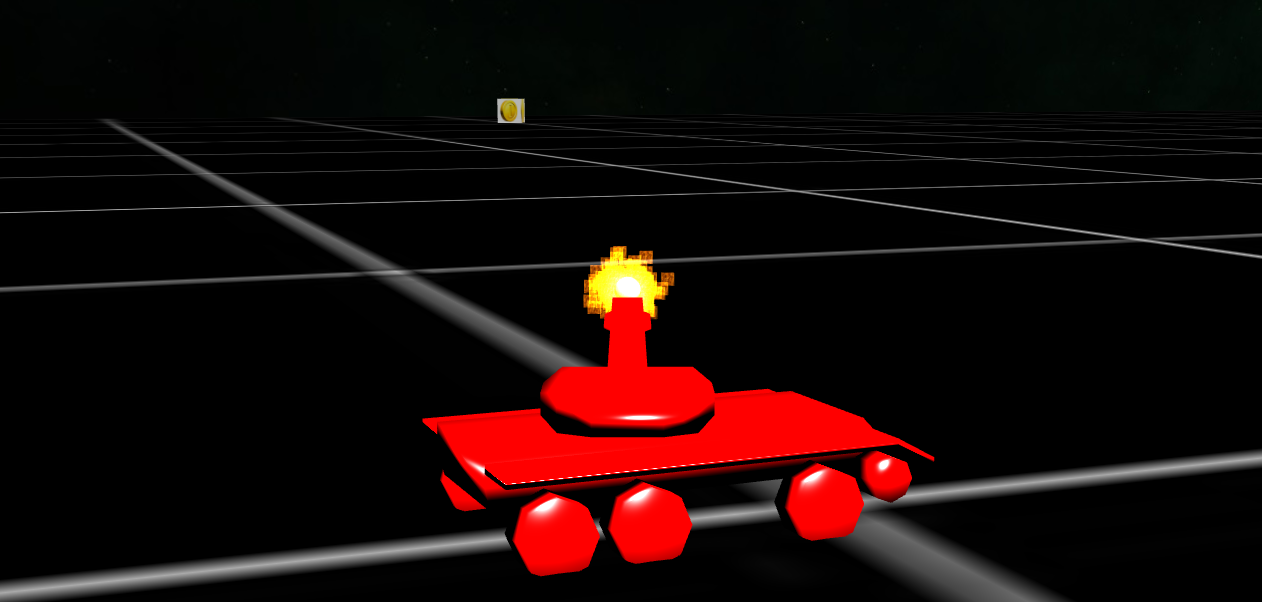
\includegraphics[width=\textwidth]{images/turret1.png}
\end{minipage}
\hfill
\begin{minipage}[t]{0.45\textwidth}
\center
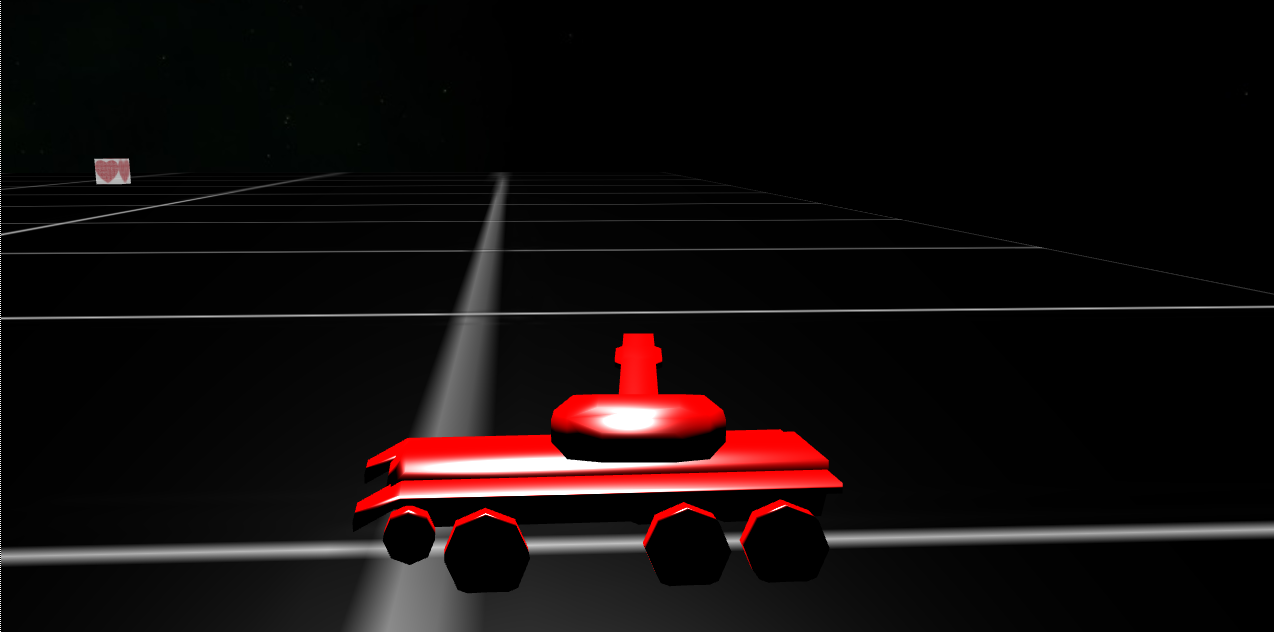
\includegraphics[width=\textwidth]{images/turret2.png}
\end{minipage}
\caption{Two pictures depicting two different orientations of the tank turret.}
\label{img:turretOrientation}
\end{figure}

One of the most difficult features in the game to implement was undoubtedly the animation of the turret. In this case, I did not use any key frame animation since I want the player to be able to rotate the turret differently from time to time following the mouse movements and doing so with a predefined set of values for each frame of the animation would have been impossible. Then, the turret animation is handled in a separate function.\\
To rotate the turret we need know exactly how much we have to rotate the tank turret to match the direction of the follow camera as in figure \ref{img:turretOrientation}. Babylon.js comes in help with a very simple function to obtain the position that is right in front of the camera at a given distance: \textit{camera.getFrontPosition(distance)} \footnote{\url{https://doc.babylonjs.com/api/classes/babylon.followcamera\# getfrontposition}}. This function returns a vector which represents the position in front of the camera at a given distance. We call \(\beta\) the angle between the position of the camera and the position of the \textit{front vector}.The front vector is a vector that points towards the front direction of the tank. The tank front vector is always updated whenever the tank is translated or rotated. To obtain this angle we need to make few considerations.
To perform this computation, we need two vectors mainly: the position of the object in front of the tank and the follow camera position. The difference between these two vectors gives the vector that joins them. The angle between the camera position and the vector difference is \(\beta\), the angle we are looking for. We know also that the x component of the difference vector is the sine of the angle \(\beta\) and the z component is the cosine of the angle \(\beta\). Given \(d= (d_{x},d_{y},d_{z})\) the difference vector, to obtain \(\beta\) we simply need to solve this simple non linear system of equations:
\begin{equation}\label{eq:animateTurret}
\begin{cases}
\sin(\beta) = d_{x}\\
\cos(\beta) = d_{z}
\end{cases}
\end{equation}
By computing the ratio of the two equations, we know that 
\begin{equation}\label{eq:beta}
\beta = \arctan\left(\frac{d_{x}}{d_{z}}\right)
\end{equation}
For simplicity, I want to rotate the turret just along the y axis regardless the orientation of the camera along the x and the z axes. Then, we slightly modify the difference vector replacing the y component of the difference vector to 0. Computing \(\beta\) is not sufficient as this will cause the turret to be rotated also when the tank turns left or right. I want the turret to be rotated if and only if the camera moves. Then I need to slightly adjust the angle to take into account the rotation angle of the tank. We may call this angle \(\gamma\).



\begin{figure}[H]
\begin{minipage}[t]{0.77\textwidth}
\center
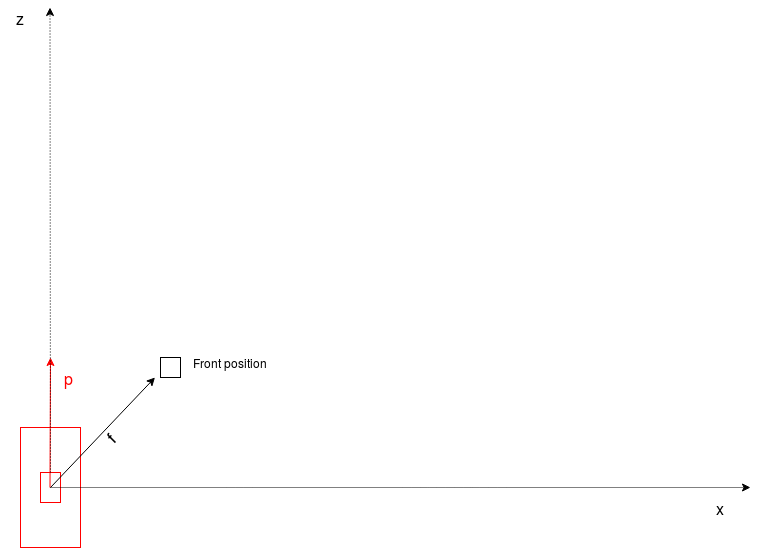
\includegraphics[width=\textwidth]{diagrams/turretChart.png}
\end{minipage}
\hfill
\begin{minipage}[t]{0.77\textwidth}
\center
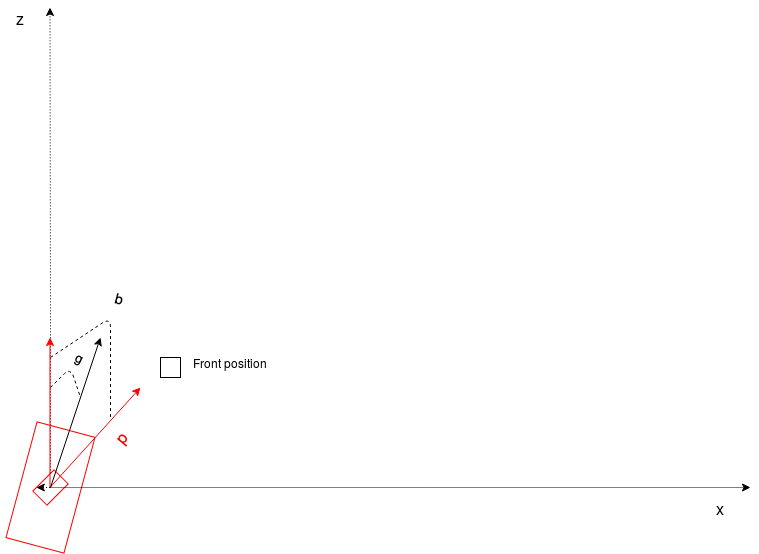
\includegraphics[width=\textwidth]{diagrams/turretChartRot.png}
\end{minipage}
\caption{Simple scheme of the two phases of the tank turret roation. To accomplish the rotation I must consider also the tank rotation represented in this figure by the angle \textit{g}. \textit{b} is \(\hat{\beta}\), the angle I want to compute to perform the rotation.}
\label{img:turretChartOrientation}
\end{figure}



Suppose I turn right of \(\frac{\pi}{4}\) radians which correspond to a rotation \(-\frac{\pi}{4}\) along the y axis for the camera position vector. If I solve the system  in the equation \ref{eq:beta}, I obtain an angle which is offset by \(\gamma\). To get rid of this effect, I just need to subtract \(\gamma\) from  \(\beta\) obtaining:
\[\hat{\beta} = \beta - \gamma\]
Once I obtain \(\hat{\beta}\) we simply rotate the turret along the y axis by \(\hat{\beta}\) radians and the job is done. Since the turret is a parent node of the cannon in the hierarchical model, rotating the turret will inevitably rotate the cannon that is the final effect we want to achieve in this animation. 
\subsection{Dealing with collisions}
Babylon.js implements a very simple collision system that, if enabled avoid that two meshes fully intersect. To enable the collision system we simply have to set a boolean variable in the mesh object. So not all the meshes have the collision system enabled. I created a simple bounding box that surrounds the tank model and moves togheter with it. The bounding box dimensions are set so that each tank is completely surrounded by its bounding box and the other tanks can't intersect it [figure \ref{img:boundingBoxes} ]. Whenever we move the tank, we also move the bounding box so that the tank and the box become a unique moving body \footnote{See the tank.move() function documentation in \textit{tank.js}}.

\subsection{The hit bounding box}

\begin{figure}[H]
\begin{minipage}[t]{0.5\textwidth}
\center
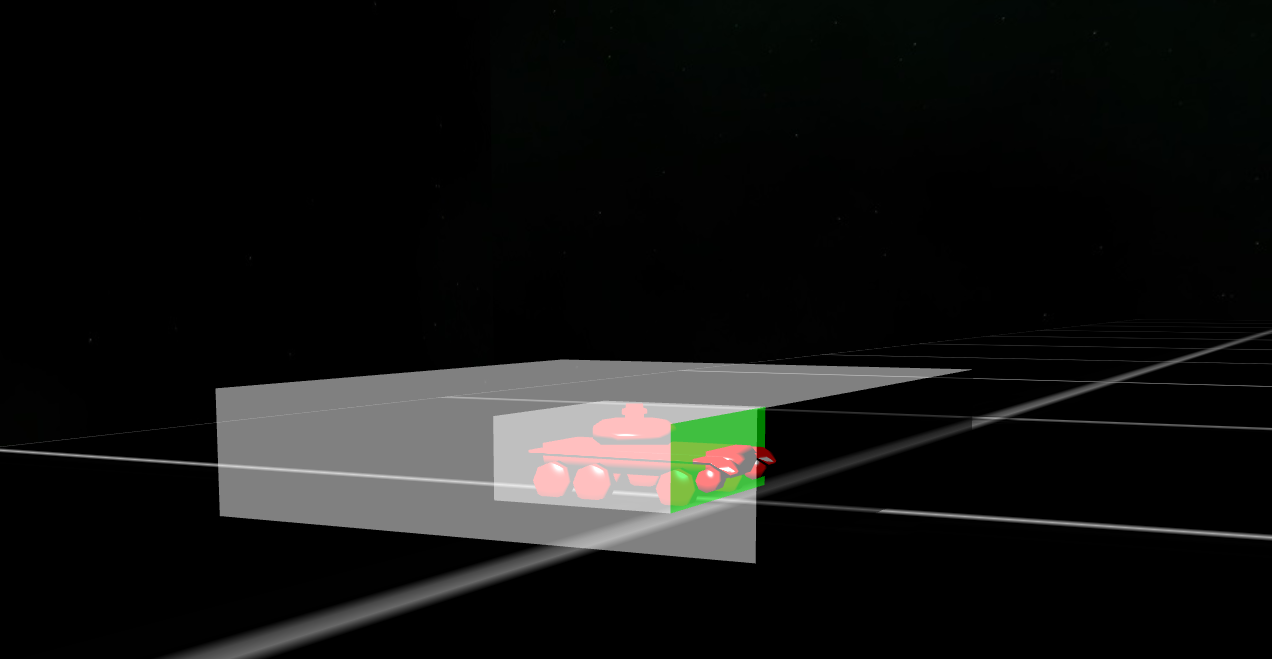
\includegraphics[width=\textwidth]{images/boundingBoxes.png}
\end{minipage}
\hfill
\begin{minipage}[t]{0.5\textwidth}
\center
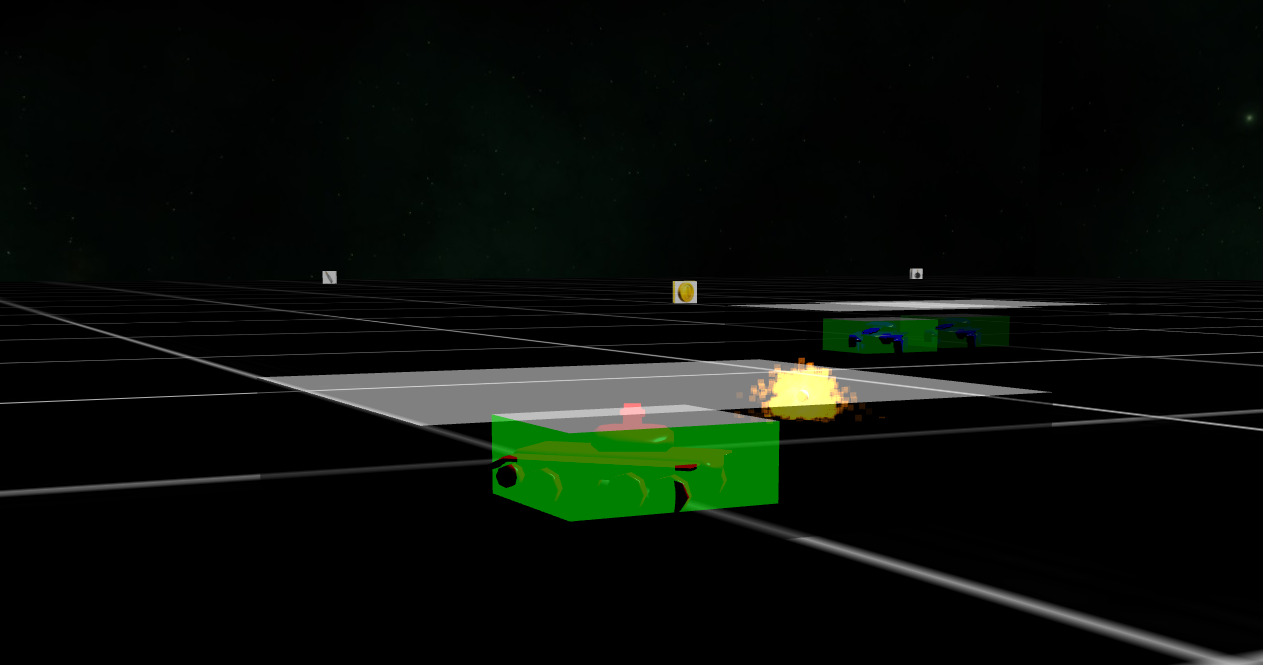
\includegraphics[width=\textwidth]{images/boundingBoxes2.png}
\end{minipage} 
\caption{The hit (green) and the collision (gray) bounding boxes of the models.}
\label{img:boundingBoxes}
\end{figure}


In order to handle cannon ball hits, I use another smaller bounding box which form now on, I will call the \textbf{hit bounding box} [figure \ref{img:boundingBoxes} ]. The hit bounding box is much smaller as we do not want the player to experiment any \textit{phantom range damage}
\footnote{In video games, a \textit{phantom range} is a very annoying problem that arises whenever the hit box/boxes of a given model is/are far larger than the model itself. This will cause the players to experiment damage from blows that actually hit a region in the space which is clearly far from the the player character, causing frustration and ruining the game experience. Actually many AAA games are recognized to have this problem.}

that will make the whole gaming experience quite frustrating. When moving the tanks, we handle the hit bounding box in the same way we handled the collision bounding boxes moving them toghether with the tank. In the final version of the game, both the two bounding boxes will be invisible, but still be rendered and considered by the Babylon.js collision engine.

\section{The player tank}
As I said before, the player tank is a mesh imported from a website. Choosing an appropriate mesh which allowed me to animate the various components was quite a difficult task. There are a lot of high quality meshes available online. The problem was substantially the fact that those meshes cannot be completely animated as the various part are not directly accessible by Babylon. Importing a highly detailed model of a world war 2 tank and not being able to animate the crawler is quite disappointing. Luckily, I managed to find this very basic tank model which comes as a collection of boxes of a given size arranged in such a way that they resemble a tank. Despite the minimal design the model is functional: all the boxes can be accessed and animated independently from one another.\\
\subsection{Animating the model}
\subsubsection{Moving the tank}
Once imported, I needed to define some basic interactions. I did not provide the ground to any form of friction force, so I had to find a way to simulate acceleration, braking and steering. \\
The first thing I did was to provide the player with a more \textit{game like} movement system: instead of using the arrow keys or the left mouse button to move the tank, I addressed WASD for that purpose. Achieving this is quite straightforward through javascript event listener. First a global \textit{WASD handler} object is istantiated to  which button of the WASD grid is pressed. Secondly, we enabled a javascript event listener on the WASD keys that trigger a boolean flag in the handler when the button is pressed. This results in the tank moving forward when W is pressed, backward when the S button is pressed and to rotate clockwise and counter clockwise when D and A are pressed respectively. Movement is done through the \textit{moveWithCollision} 
\footnote{\url{https://doc.babylonjs.com/babylon101/cameras,_mesh_collisions_and_gravity}.}
Babylon js built-in functions and rotation is applied using the \textit{rotate} function of the Babylon.Mesh object. It a very simple system and it works but it is not enough. We want the tank to actually accelerate up to a predefined top speed when W is pressed and we want the tank to actually \textbf{break} when the S button is pressed. To accomplish this we define a parameter \textit{speed} for the tank object. The speed parameter regulates the movement speed of the tank. At the starting point the speed is set to 0. When the player presses W, the speed parameter is increased by 0.01 and this value is multiplied to the translation vector that defines the movement speed of the tank. On the contrary, when S is pressed the speed parameter is decreased by the same value. Once the speed parameter becomes negative, the tank starts moving backwards. Pressing A or D does not affect the tank speed parameter. If the player stops pressing one of the WASD buttons the tank immediately freezes. \\
Moving the tank should cause the wheels to rotate as they get in contact with the ground. To accomplish this we rotate along the x axis all the wheels clockwise when the speed parameter is greater than zero and counter clockwise when the tank moves backward.\\
The wheel rotation is performed at every render loop iteration.\\

\subsubsection{External color and design}
The player tank belongs to the red team by default. We then need to find a way to distinguish the player tank from the opponent tank team. This can be easily accomplished by applying a red colore material object to the player tank surface. In Babylon.js a standard material will have four color components that will react differently from light sources: 
\begin{itemize}
\item A diffuse colour component that will react properly with the diffuse component of the light sources.
\item A specular colour component that will react properly with the specular component of the light sources.
\item An ambient colour component that will react properly with the ambient component of the light sources.
\item An additional emissive component that will render a colour which is independent of the light sources that are present in the scene.
\end{itemize}
For design purposes we set the diffuse colour and the emissive colour of the player tank to red. The diffuse component is intended to make the tank material sensible to react to the light sources, the second one to render a red colour even if in the scene there is no light source with a red diffuse component or there is no light source at all.
\subsection{Shooting}
The main feature of this game is to simulate an arena battle between two team of tanks. So there must be a way for both the player and the opponent tanks to cause some damage. In this game the tanks will have two weapons mainly: the \textbf{cannon} and the \textbf{machine gun}.\\
\subsubsection{The cannon}
The cannon is the main weapon of the tanks. It can shoot fire cannon balls towards the enemy and cause a damage of exactly 2 life points. The cannon ball source is placed directly in front of the tank cannon. Whenever the player shoots a cannon ball the program retrieves both the position and the orentation of the tank cannon and set it as the spawn position of the cannon ball. \\
The cannnon ball is rendered using a simple sphere mesh and has a red colour to simulate the heat of the thrown cannon ball. \\



\begin{figure}[H]
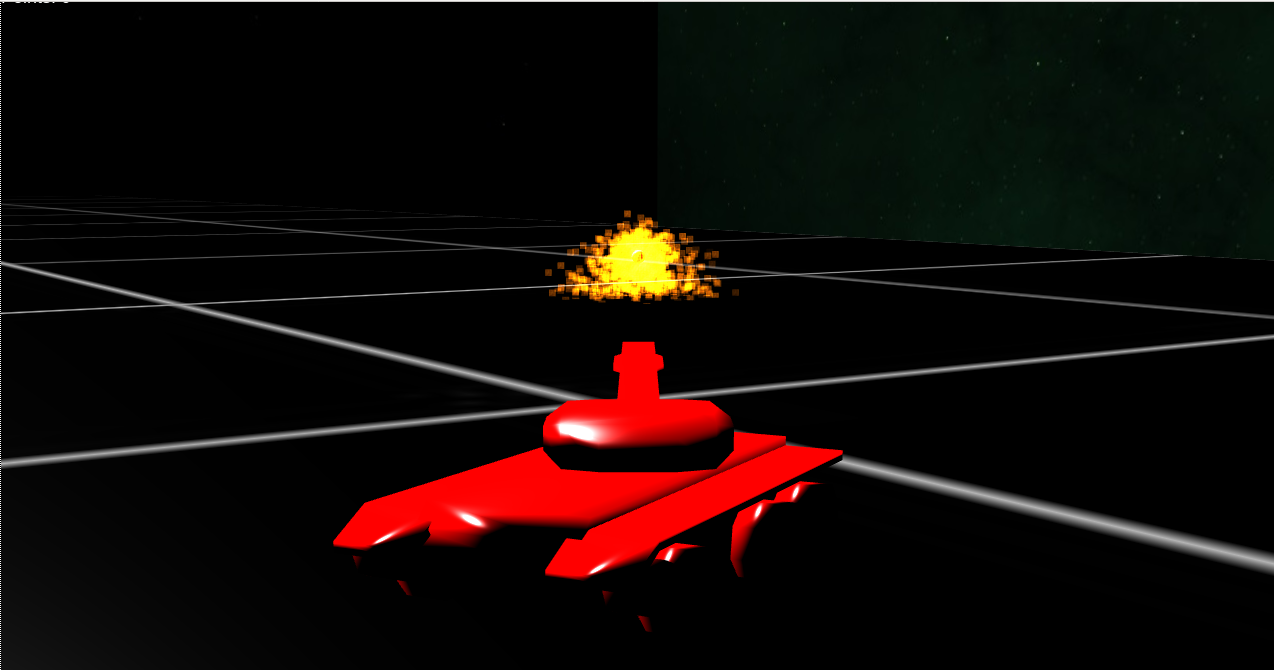
\includegraphics[width=12cm]{images/cannonBall2.png}
\caption{This image shows the cannon ball and the fire particle system.}
\label{img:cannon}
\end{figure}




In order to simulate a fire ball effect, we used a properly tuned particle system to simulate fire. To give the particles a spherical trajectory, I used also a \textit{sphere emitter} object which sets a \textit{spherical emission region} centered in the emitter mesh. The emitter source of the particle system is the sphere representing the cannon ball and we set the emission region to move toghether with the cannon ball as shown in figure \ref{img:cannon}.\\
The maximum lifetime of the particles is set to a few seconds and a fire texture has been applied to them.\\
The ball can react to other meshes in the scene thanks to the physics engine. In order to throw the cannon ball toward the direction pointed by the cannon ball we simply apply a physic impulse. The impulse is applied to the center of the sphere mesh and points towards the direction of the cannon turret. The strength of the impulse is a parameter of the Tank class and is tuned to create a balanced shooting system. The physics engine, then, applies an earth like gravity  (\(g_{y} = -9.81 \ \frac{m}{s^{2}}\)) to the cannon ball so that the latter will have a parabolic trajectory towards the shooting direction. The ball then reacts with the environment in the following way:
\begin{itemize}
\item  If the cannon ball intersects the hit box of one of the opposite team tanks (friendly fire is not allowed), it will explode and cause damage to the target tank. 
\item If the cannon ball does not hit anything after 4 seconds it disappears and the corresponding mesh is disposed for efficiency reasons.
\end{itemize}
The code associated with the cannon ball action manager is executed when the cannon ball intersects the \textbf{hit bounding box} of the opponent tank. The action code stops the cannon ball particle system, disposes the cannon ball and starts another particle system which emits particles directly from the opponent tank body to simulate the explosion. The function also reproduces an explosion sound once the cannon ball hits the opponent tank.
\subsubsection{The machine gun}
Very similar to the cannon ball, it represents the secondary weapon of the tanks. The machine gun is very easy to use but deals less damage. \\



\begin{figure}[H]
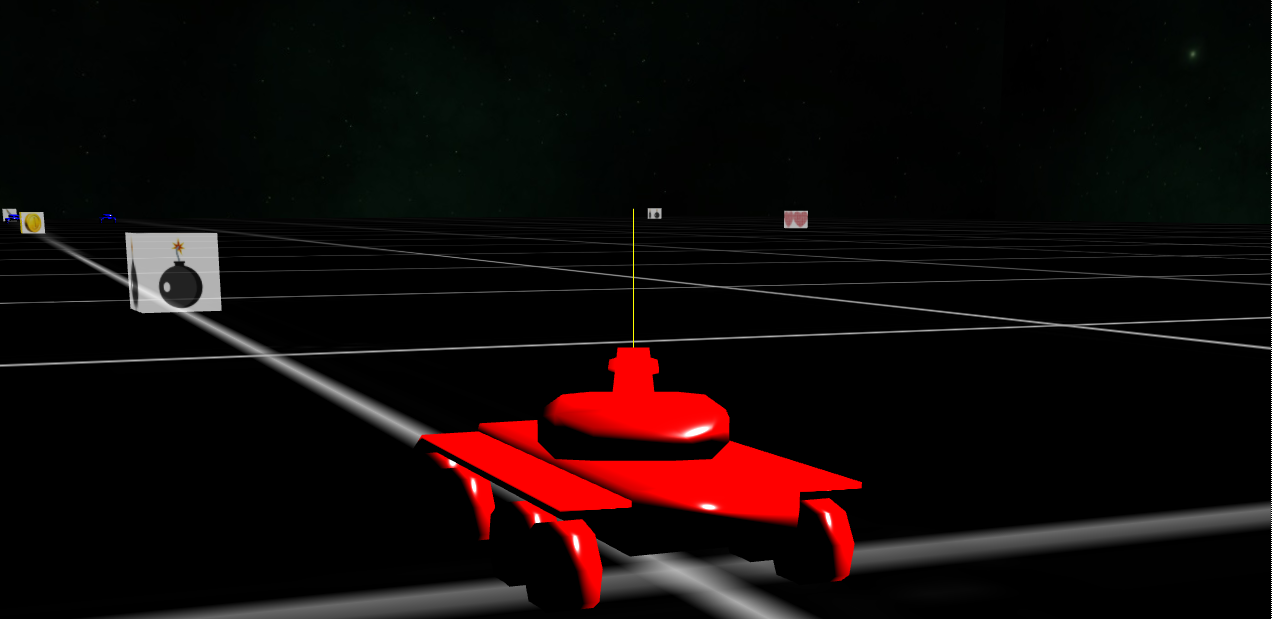
\includegraphics[width=12cm]{images/machineGun.png}
\caption{This image shows the tank using the machine gun.}
\label{img:machineGun}
\end{figure}

To simulate the machine gun bullets I used Babylon.js \textit{rays}. In Babylon js a ray is, as the name suggets, a line in the context of a scene. To throw rays, I need to specify an origin, a direction and a length. By default, rays are invisible, but thanks to the \textit{ray helper} I managed to make them visible as shown in figure  \ref{img:machineGun}. A Babylon.js ray intersects objects and the user can define callbacks that will be executed whenever an object is intersected. Obviously, we may not want this callback to be executed when the intersected mesh is, for example, the skybox. Babylon.js ray helpers allows the user to define precisely which meshes should be taken into account by setting appropriate boolean expressions. In this case, only the meshes which belongs to the opponent tanks should trigger this callback. Fortunately, can be immediately spotted by inspecting their names. All the tank model meshes have a name that contains the string "Box" ("clone\textunderscore 1.Box14.Box15","Box7" etc ...), thus a simple solution to this problem is to use javascript \textit{regular expressions}. If the target mesh name is the format described above, then it matches some regular expressions and when the ray intersects it, the proper callback will be triggered. \\
The callback structure is very simple. It decreases the target tank health and performs a simple test: if the health of the target tank is less or equal than 0, the target tank dies, otherwise nothing happens.
\subsubsection{The tanks death}
If the tank health reaches a value of 0, the tank must disappear from the scene. If it is the case, then a special death function is performed. \\
The tank death should be handled with care. When it comes the time of disposing a tank I must be sure that, not only the model will disappear, but also that all the objects that are associated to it are released to \textbf{free memory space}. Then, before disposing the tank meshes I ensure that:
\begin{itemize}
\item All the tank particle systems are shut down.
\item All the tank particle systems are disposed.
\item The hit and collision bounding boxes are disposed.
\item The tank meshes are disposed.
\end{itemize}
After destroying all the tank components, the function has a different behaviour depending on the fact that the target tank is the player tank. If it is the case, then another routine is called and a \textit{game over} menu is displayed allowing the player to do nothing but to go to the main menu to start another game.\\
If the eliminated tank is an opponent tank, then a timeout of 5 seconds is set, after which the opponent tank is respawned. To handle the respawn of opponent tanks, I first retrieve its spawn point, which has been previously stored inside the obejct representing the tank. Then I create another clone of the tank model, and move it to its spawn position so that it can rejoin the fight.

\section{The opponent tanks}
The opponent tanks are handled inside a loop that is executed at every rendering iteration. In this loop each tank execute its policy.
\subsection{The opponent tank policy}
Currently the opponent tanks adopt a very simple random aggressive policy: at every rendering iteration a random number is generated. If this number is greater than a certain parameter which is defined by the tank policy, then the tank will shoot towards the player otherwise, it won't shoot. To decide whether the blue tank will use the cannon or the machine gun another random number is generated. If the value is greater than a certain value, then the tank will switch weapon, otherwise, it keeps shooting with the same weapon. \\
The opponent tanks are designed to do nothing but to kill the player. They will constantly follow the player tank trying to destroy it. For simplicity, the opponent tanks will never run out of bullets so they can potentially shoot for an infinite time, forcing the player to be dynamic trying to avoid the opponent bullets.\\
\subsection{Movement}
I handled the blue tanks movement in a separate function. I set the tank to always point towards the direction of the player tank and to follow it with a fixed speed. To accomplish this, we compute a difference between two vectors: the tank \textit{front vector} and the opponent tank \textit{front vector}. \\
The difference between these two vectors returns the vector that joins them. The goal of this operation is to obtain the angle \(\alpha\) between the opponent front vector and the difference vector. To do that I needed to make few considerations: I know that the projection along the x axis of the difference vector represents the sine of the angle, whereas the projection along the z axis represents the cosine of the angle. To obtain the alpha angle I should solve the following non linear system:
\begin{equation}\label{eq:followTank}
\begin{cases}
\sin(\alpha) = d_{x}\\
\cos(\alpha) = d_{z}
\end{cases}
\end{equation}
By computing the ratio of the two equations, I obtain: 
\begin{equation}\label{eq:alpha}
\alpha = \arctan\left(\frac{d_{x}}{d_{z}}\right)
\end{equation}
It is not sufficient to compute \(\alpha\). Since I used the negative front vector of the blue tanks to compute the angle, if I perform a rotation of \(\alpha\) radians along the y axis, the blue tank will point exactly in the opposite direction of the player tank as shown in figure  \ref{img:threeOrientations}. To obtain the angle we are looking for, then, we need to sum \(\pi\) to the angle \(\alpha\). Then \[\hat{\alpha} = \alpha + \pi\]
Once I compute \(\hat{\alpha}\), I rotate the blue tank along the y axis by \(\hat{\alpha}\) radians, replace its front vector with the difference vector and move the tank in the direction defined by the new front vector.\\



\begin{figure}[H]
\begin{minipage}[t]{0.6\textwidth}
\center
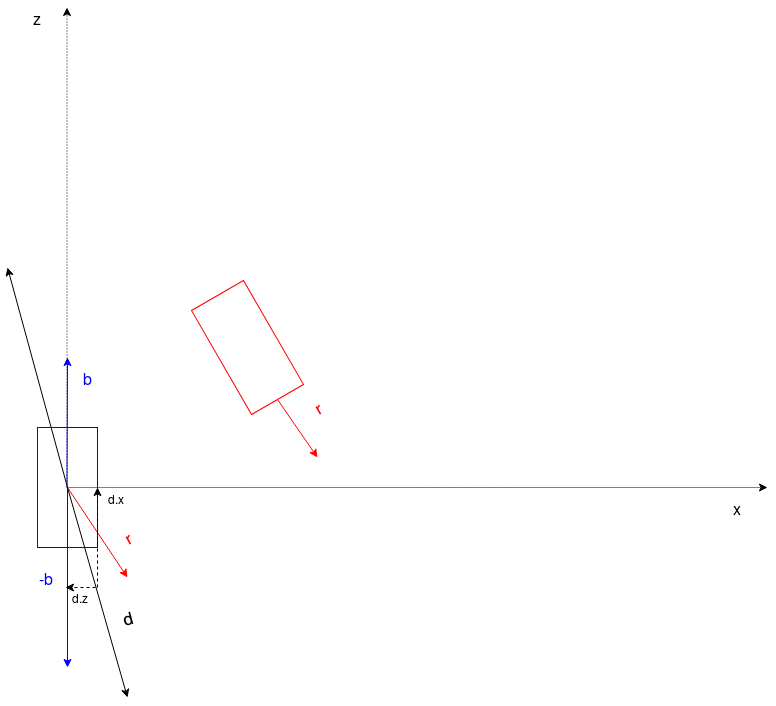
\includegraphics[width=\textwidth]{diagrams/chart.png}
\end{minipage}
\hfill
\begin{minipage}[t]{0.6\textwidth}
\center
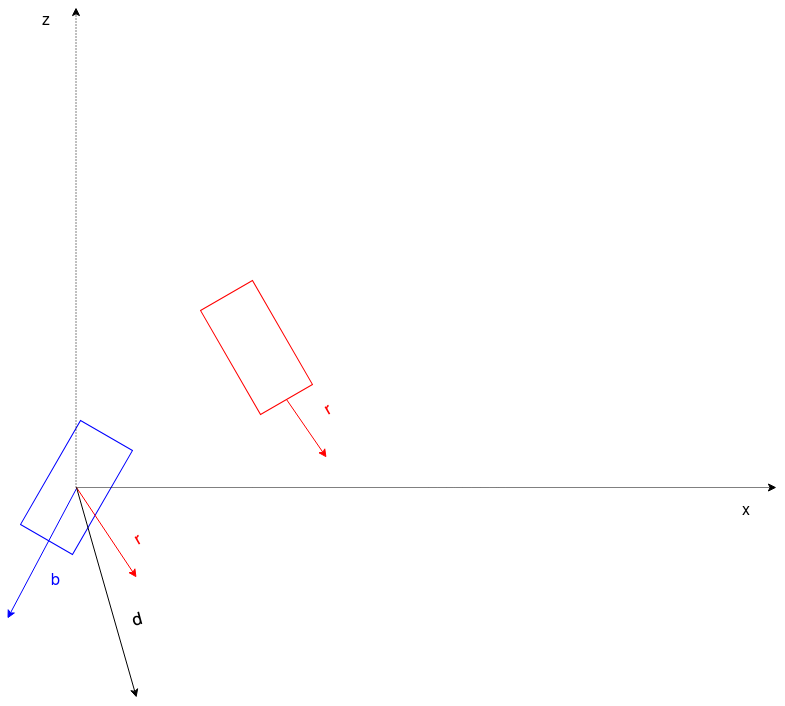
\includegraphics[width=\textwidth]{diagrams/chartFirstRot.png}
\end{minipage}
\begin{minipage}[t]{0.6\textwidth}
\center
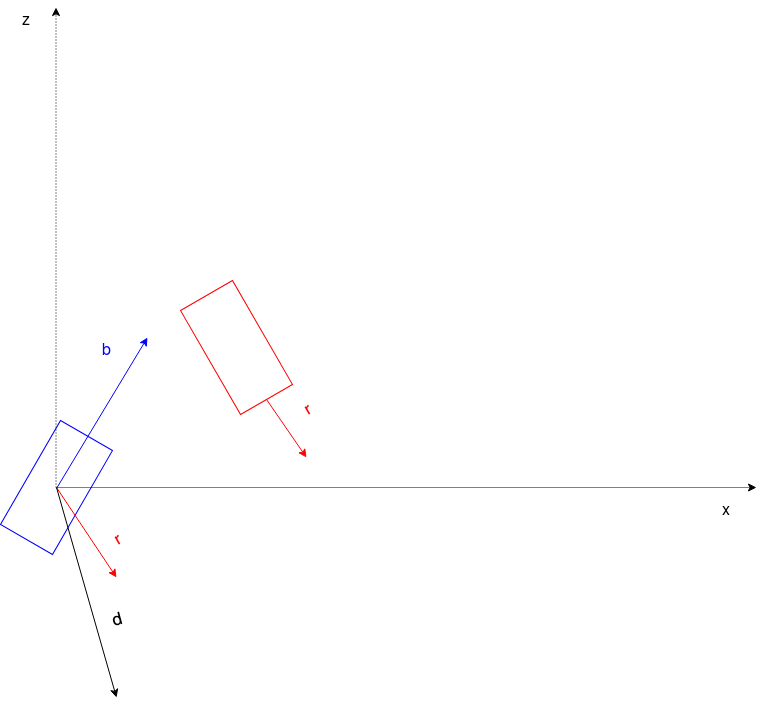
\includegraphics[width=\textwidth]{diagrams/chartSecondRot.png}
\end{minipage}
\caption{Scheme of the three rotations. In the first image, the difference vector \(d\) si computed. In the second one the blue tank is rotated clockwise by \(\alpha\) radians. In the third image \(\hat{\alpha}\) is computed and the final rotation is performed.}
\label{img:threeOrientations}
\end{figure}




By continuously doing this in the render loop, the blue tanks will never stop following the hero tank. 
\section{The game}\label{sec:theGame}
This section aims at illustrating a user manual of the game. 

\subsection{Description}
The game is a simple third person arena game in which the player tank and the blue tank team fight to the death. The arena is a simple flat map in which the tanks are able to move. Both the player tank and the opponent team can shoot with two weapons: the cannon and the machine gun. The player tank is also able to restore life points, to collect cannon and machine gun bullets from the loot boxes that float in certain positions of the map. The goal of the player tank is to collect a sufficient number of points to win the stage. The amount of points needed to win changes with the game difficulty which can be either \textbf{easy} or \textbf{hard}. In easy mode the player needs to collect 5 points whereas in hard mode the points needed are 10. The player can collect points by picking the \textit{point loot boxes} which are easily spotted by a big gold coin texture. In easy mode, there are two point loot boxes that respawn after 5 seconds whereas in hard mode there is just one loot box making more difficult for the player to win the stage. The respawn time of the point loot box remains the same. \\
The player will face an opponent team of blue tanks that have the only purpose of killing him. Also the number of opponent tanks varies toghether with the game difficulty. In easy mode, there are just two tanks, in hard mode there are four of them. In each of the two game difficulties, the blue tanks will have infinite ammo for their weapons whereas the player tank has just few limited amount.
\subsection{Commands}
At the beginning of the game the player will be placed in front of the main menu. In this menu, he can choose the difficulty of the game which can be either easy or difficult, enable or disable the sound and start a new game. \\
When the match begins, the player starts with the red tank. The tank can be moved pressing WASD and the turret can be rotated by simply moving the mouse. Press the left mouse button on the canvas to have the mouse pointer locked inside the game and fully control the tank turret. Move the mouse to rotate the turret. Make sure that the turret points towards the enemy tanks, as otherwise you will waste ammo.\\
Press the left mouse button to shoot. You can shoot with two different weapons: the cannon and the machine gun. To use the cannon, press "1" whereas to switch to the machine gun, press "2". You can always terminate the game by pressing "m".
\subsection{Player guide} 
The game is very simple, but the very aggressive blue tank policy may cause the player to rapidly lose life points without even noticing it. A simple strategy to win a match could be the following. \\


\begin{figure}[H]
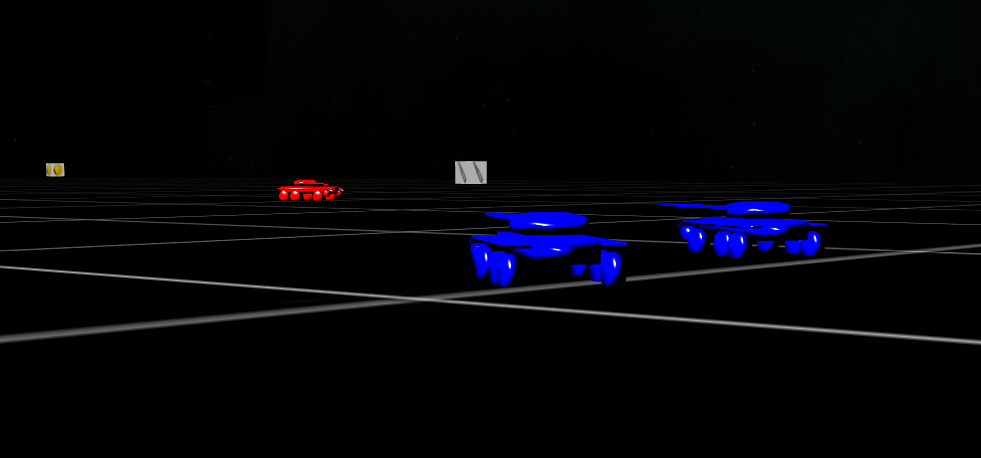
\includegraphics[width=12cm]{images/game.png}
\caption{Screenshot of the game scene.}
\label{img:machineGun}
\end{figure}

Move continously around the map. Keep turning left and right to avoid opponent cannon balls and never stop moving for any reason. Avoid being exactly in front of the opponent tanks as this will probably cause their cannon balls to hit the player tank. Remeber: your tank starts with 10 life points, so 5 cannon balls are more than enough to hunt you down. Always focus of picking the loot boxes. Aim at the point loot boxes first, but if you see your life to go below 4 points, change your objective and try to pick some health loot boxes.\\
Hunt down few opponent tanks if you can,exspecially on hard difficulty, but never stop hunting the point loot boxes. Keep in mind that, differently from you, they have infinite cannon balls and machine gun bullets, so, sooner or later, they will manage to destroy you expecially if you play careless . \\
The cannon is certainly the most effective weapon, but you starts with just 10 cannon balls. Moreover, you have to consider that the cannon balls are heavy and are affected by gravity. Then shooting with the cannon will make you cause more damage, but you will be less precise. On the contrary, the machine gun is a weaker but indeed a  more precise weapon. Mix them to achieve letalithy.






\end{document}